\documentclass[12pt]{article}

% Packages for math and formatting
\usepackage[utf8]{inputenc}
\usepackage{amsmath, amssymb, amsthm}
\usepackage{geometry}
\usepackage{enumitem}
\usepackage{hyperref}
\usepackage{mathtools}
\usepackage{epigraph}
\usepackage{tikz}
\usetikzlibrary{arrows.meta, decorations.pathmorphing, positioning}

% Page setup
\geometry{margin=1in}

% Theorem-like environments
\newtheorem{theorem}{Theorem}[section]
\newtheorem{proposition}[theorem]{Proposition}
\newtheorem{lemma}[theorem]{Lemma}
\newtheorem{corollary}[theorem]{Corollary}
\theoremstyle{definition}
\newtheorem{definition}[theorem]{Definition}
\newtheorem{problem}[theorem]{Problem}
\theoremstyle{remark}
\newtheorem{remark}[theorem]{Remark}
\newtheorem{example}[theorem]{Example}

% Custom commands
\newcommand{\R}{\mathbb{R}}
\newcommand{\N}{\mathbb{N}}
\newcommand{\Q}{\mathbb{Q}}
\newcommand{\Z}{\mathbb{Z}}
\newcommand{\C}{\mathbb{C}}
\newcommand{\PP}{\mathbb{P}}
\newcommand{\D}{\mathbb{D}}
\newcommand{\HH}{\mathbb{H}} % upper half-plane

% Operator names
\DeclareMathOperator{\Aut}{Aut}
\DeclareMathOperator{\FractLin}{FractLin}
\DeclareMathOperator{\ord}{ord}
\DeclareMathOperator{\Res}{Res}
\DeclareMathOperator{\SL}{SL}

\title{Elliptic Functions, Part 2}
\author{Joe}
\date{October 8, 2025}

\begin{document}
	
	\maketitle
	
	\epigraph{You have to ask many times before you get to the right question.}{\textit{Prof. MOK Ngaiming}}
	
	\tableofcontents
	\vspace{1em}
	
	Recall the universal properties of elliptic functions:
	
	\begin{theorem}[General Properties of Elliptic Functions]
		Let $\Pi$ be a fundamental domain for $X = \C/L$. Suppose $f$ is an elliptic function such that $f$ has no zeros nor poles on $\partial \Pi$. Then the following holds true:
		\begin{enumerate}
			\item[(a)] $\displaystyle \sum_{a_k \in P(f|_\Pi)} \Res(f; a_k) = 0.$
			
			\item[(b)] $\displaystyle \sum_{a_k \in Z(f|_\Pi)} \ord_{a_k}(f) + \sum_{b_l \in P(f|_\Pi)} \ord_{b_l}(f) = 0.$
					\item[(c)] $\displaystyle \sum_{a \in \Pi}' \ord_a(f) \cdot a \equiv 0 \pmod{L}.$
		\end{enumerate}
	\end{theorem}
	
	From (a), it follows that there cannot exist $f \in M(X)$ such that $f$ has a simple pole at some $x \in X$ and no other poles; otherwise,
	\[
	\sum_{x \in \Pi}' \Res(f; x) = \Res(f; a) \neq 0,
	\]
	contradicting~(a).
	
\section{Weierstrass $\wp$-function}

Recall the \emph{Eisenstein series}:  

\begin{corollary}[Eisenstein Series Construction]\label{cor:eisenstein}
	When $k \geq 3$, we can define the \emph{Eisenstein series} by
	\[
	E_k(z) = \sum_{w \in L} \frac{1}{(z+w)^k},
	\]
	where $E$ stands for Eisenstein.
	
	\noindent The function $E_k$ has a pole of order $k$ at lattice points and no other poles. Moreover, $E_k$ is doubly periodic with respect to $L$, and hence descends to a meromorphic function on the elliptic curve $X = \C / L$.
\end{corollary}

When $k \geq 3$, we have $\operatorname{ord}_0(E_k) = -k$.  
The Weierstrass $\wp$-function satisfies the fundamental relation
\[
\wp'(z) = -2E_3(z).
\]\\
\underline{Observation}: If $f$ is elliptic with respect to $L$, then $f'$ is also elliptic with respect to $L$. \\

\noindent \underline{Question}: What about the converse? \\

Suppose $f$ is meromorphic on $\C$ and $f'$ is elliptic with respect to $L$. 

\noindent \textbf{Question 1.} Is $f$ elliptic?

Consider $\omega \in L$, and define
\[
h_{\omega}(z) = f(z+\omega) - f(z), \quad 
h'_{\omega}(z) = f'(z+\omega) - f'(z) = 0.
\]
By hypothesis, we have $h_{\omega}(z) = C_{\omega}$ for some constant $C_{\omega} \in \C$.
Moreover,
\[
C_{\omega+\omega'} = C_{\omega} + C_{\omega'}.
\]



\noindent \textbf{Question 2.} Let $g$ be elliptic with respect to $L$, i.e.
\[
g(z+\omega) = g(z), \quad \forall\, z \in \C,\, \forall\, \omega \in L.
\]
Consider
\[
\begin{cases}
	\exists\, f \in \mathcal{M}(X) \text{ such that } f' \equiv g? \\[0.3em]
	\text{If such } f \text{ exists, is it elliptic with respect to } L?
\end{cases}
\]

For the first part, we can try to integrate. 
Take $z_0 \in \C$ where $g$ is holomorphic, and let $\gamma$ be a piecewise $C^1$ path joining $z_0$ to $z$. 
Then we ``define''
\[
f(z) = \int_{\gamma} g(\xi)\, d\xi.
\]
Without assuming the ellipticity of \( g \), here is the complete answer.  
Let \(\{a_k\}\) be the poles of \( g \).  
Let \(\Gamma_k^0\) be a small loop around \(a_k\), and set \(a_k \rightarrow a_k + \varepsilon e^{i\theta}\), where \(\theta \in [0, 2\pi]\).

If there exists \(f\) such that \(f' \equiv g\), then we must have
\[
\int_{\Gamma_k^0} g(\xi)\, d\xi = 0,
\]
where \(\Gamma_k^0\) is an anticlockwise loop encircling \(a_k\).

Now, let \(\Gamma_k - \Gamma_k^0\) bound a domain \(\Omega\), i.e.
\[
\partial \Omega = \Gamma_k - \Gamma_k^0.
\]


\begin{center}
	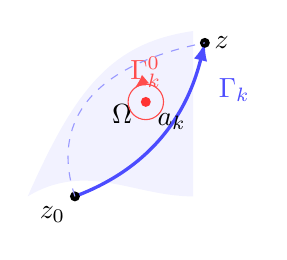
\begin{tikzpicture}[scale=1.5, >=latex]
		
		% Shaded region Ω (to the left of Γ_k)
		\fill[blue!5] (-1.2,-0.1) .. controls (-0.8,0.8) and (-0.5,1.2) .. (0.2,1.3)
		-- (0.2,-0.1) .. controls (-0.3,-0.1) and (-0.7,0.2) .. cycle;
		\node at (-0.4,0.6) {$\Omega$};
		
		% Γ_k curve from z0 to z
		\draw[very thick, blue!70, ->] (-0.8,-0.1)
		.. controls (0.0,0.2) and (0.2,0.8) .. (0.3,1.2);
		\node[blue!70] at (0.55,0.8) {$\Gamma_k$};
		
		% Starting point z0
		\fill ( -0.8,-0.1 ) circle (1.2pt);
		\node[below left] at (-0.8,-0.1) {$z_0$};
		
		% Endpoint z
		\fill (0.3,1.2) circle (1.2pt);
		\node[right] at (0.3,1.2) {$z$};
		
		% Pole a_k and small loop Γ_k^0 around it
		\fill[red!80] (-0.2,0.7) circle (1.2pt);
		\node[below right=1pt of {(-0.2,0.7)}] {$a_k$};
		\draw[red!70,->] (-0.2,0.7) circle [radius=0.15];
		\node[red!70] at (-0.2,0.95) {$\Gamma_k^0$};
		
		% Orientation of small loop
		\draw[->, red!70, thick] (-0.2,0.85) arc[start angle=90, end angle=130, radius=0.15];
		
		% Dashed arc suggesting rest of Ω boundary
		\draw[dashed, blue!40] (-0.8,-0.1)
		.. controls (-1.0,0.5) and (-0.7,1.0) .. (0.3,1.2);
		
	
		
	\end{tikzpicture}
\end{center}
	
\begin{theorem}[Stokes' Theorem]
	Let \( M \) be an oriented smooth compact surface with boundary 
	\( \partial M \), and let \( \omega \) be a smooth differential \(1\)-form 
	defined on an open subset containing \( M \). Then
	\[
	\int_{\partial M} \omega = \int_{M} d\omega,
	\]
	where \( d\omega \) denotes the exterior derivative of \( \omega \).
	
	In particular, in the complex plane, if \( \Omega \subset \C \) and
	\( A(z), B(z) \) are smooth functions on a neighborhood of \( \Omega \), then
	\[
	\int_{\partial \Omega} \big( A(z)\,dz + B(z)\,d\bar{z} \big)
	= \iint_{\Omega} 
	\left(
	\frac{\partial B}{\partial z}
	- \frac{\partial A}{\partial \bar{z}}
	\right)
	dz \wedge d\bar{z}.
	\]
\end{theorem}

Applying this to our situation, let $\Omega \subset \C$ be a domain 
bounded by the curves $\Gamma_k$ and $\Gamma_k^0$, that is,
\[
\partial \Omega = \Gamma_k - \Gamma_k^0.
\]
For the differential form $\omega = g(\xi)\, d\xi$, Stokes' Theorem gives
\[
\int_{\Gamma_k - \Gamma_k^0} g(\xi)\, d\xi 
= \iint_{\Omega} d\big(g(\xi)\, d\xi\big).
\]
Since $g$ is holomorphic on $\Omega$ and smooth up to the boundary, 
Stokes' theorem further implies
\[
\iint_{\Omega} d\big(g(\xi)\, d\xi\big)
= \iint_{\Omega} 
\left(
\frac{\partial g}{\partial \xi}\, d\xi \wedge d\xi
+ \frac{\partial g}{\partial \bar{\xi}}\, d\bar{\xi} \wedge d\xi
\right)
= - \iint_{\Omega}
\frac{\partial g}{\partial \bar{\xi}}\, d\xi \wedge d\bar{\xi}.
\]
Because \( g \) is holomorphic, we have 
\(\dfrac{\partial g}{\partial \bar{\xi}} = 0\),
and therefore
\[
\iint_{\Omega} d\big(g(\xi)\, d\xi\big) = 0.
\]

Hence, the existence of a holomorphic function \( f \) such that 
\( f' \equiv g \) implies, by the Residue Theorem, that
\[
0 = \int_{\partial \Omega} g(\xi)\, d\xi
= 2\pi i \sum_{a_k \in \Omega} \operatorname{Res}(g; a_k),
\]
and therefore
\[
\operatorname{Res}(g; a_k) = 0
\quad \text{for all poles } a_k \text{ of } g.  \tag{$*$}
\]

Conversely, using some basic facts from topology (essentially that
integration of a holomorphic differential form defines a closed $1$‑form),
the condition \((*)\) implies that the $1$‑form
\[
\omega = g(\xi)\, d\xi
\]
is ``closed'' on the domain of definition of \( g \).
If the domain is simply connected, every closed $1$‑form is exact,
hence there exists a holomorphic function \( f \) such that
\[
df = \omega, \qquad \text{i.e.} \quad f' = g.
\]

Thus, condition \((*)\)—that the sum of residues of \( g \) in every
bounded region vanishes—ensures the global existence of a primitive \( f \)
on each simply connected component of the domain.\\

Now we come to another question. Suppose that $g$ is elliptic and that 
there exists a function $f$ such that $f' \equiv g$. 
Is $f$ necessarily elliptic?

This question depends on the particular choice of $g$.

When $k \ge 3$, recall that
\[
E_k'(z) = \sum_{w \in L} \frac{-k}{(z+w)^{k+1}}
= -k\, E_{k+1}(z).
\]
Hence, if we take $g = E_{k+1}$, then
\[
f = -\frac{1}{k}\, E_k + \text{constant}.
\]

In particular, for $k = 3$, we have
\[
E_3(z) = \sum_{w \in L} \frac{1}{(z+w)^3}.
\]
Since $\operatorname{Res}(E_3; w) = 0$ for all $w \in L$,
we know (by the existence criterion discussed earlier) that
there exists a function $f$ such that $f' \equiv E_3$.

Moreover, near the origin we may write
\[
f(z) = \frac{1}{z^2} + \cdots,
\]
and we can normalize it so that
\[
f(z) = \frac{1}{z^2} + 0 + 0 + \cdots.
\]
This leads naturally to the definition of the \emph{Weierstrass elliptic function}.

\begin{theorem}[Weierstrass $\wp$-function]
	The Weierstrass $\wp$-function associated with the lattice $L$ is defined by
	\[
	\wp(z)
	= \frac{1}{z^2}
	+ \sum_{w \in L^*}
	\left(
	\frac{1}{(z+w)^2}
	- \frac{1}{w^2}
	\right),
	\]
	where $L^* = L \setminus \{0\}$.
\end{theorem}

The function $\wp(z)$ is elliptic with respect to the lattice $L$, and satisfies
\[
\wp'(z) = -2E_3(z).
\]

One first needs to justify that the function is actually convergent in an appropriate sense.

\[
\frac{1}{(z+w)^2} - \frac{1}{w^2} 
= \frac{-z^2 - 2zw}{(z+w)^2 w^2}.
\]

Take any $R > 0$ and consider $|z| \le R.$ 
Convergence then reduces to checking that 
$\forall R > 0, \forall z \in \overline{D(R)},$
\[
\sum_{|w| \ge 2R} 
\frac{-z^2 - 2zw}{(z+w)^2 w^2} < \infty.
\]
since there are finitely many points in $L$ where $|w| < 2R$.
Now
\[
\sum_{|w| \ge 2R}
\left|
\frac{-z^2 - 2zw}{(z+w)^2 w^2}
\right|
\le
\sum_{|w| \ge 2R}
\left(
\frac{|z|^2}{|(z+w)^2 w^2|}
+
\frac{|2zw|}{|(z+w)^2 w^2|}
\right)
\le
\sum_{|w| \ge 2R}
\left(
\frac{4R^2}{|w|^4}
+
\frac{8R}{|w|^3}
\right),
\]
since $|w+z| \ge |w|/2.$

Since 
\[
\sum_{w \in L^*} \frac{1}{|w|^3} < \infty 
\quad \forall\, p \ge 3,
\]
we are done. Thus $\wp$ is convergent.

Now, is $\wp$ elliptic?
	

	
\begin{theorem}[Weierstrass]
	Let $L = \mathbb{Z}\omega_1 + \mathbb{Z}\omega_2$ be a lattice. 
	Then 
	\[
	\wp(z)
= \frac{1}{z^2}
+ \sum_{w \in L^*}
\left(
\frac{1}{(z+w)^2}
- \frac{1}{w^2}
\right)
	\]
	is an elliptic function. Moreover, it has double poles at every lattice point $w \in L$ and no other poles.
\end{theorem}

\begin{proof}
	It is obvious that $\wp$ has double poles on $L$ and no other poles. 
	What remains is to justify that $\wp$ is elliptic, i.e.,
	\[
	\begin{cases}
		\wp(z+\omega_1) = \wp(z),\\[4pt]
		\wp(z+\omega_2) = \wp(z).
	\end{cases}
	\]
	We have observed that there exist constants $C_{\omega_1}, C_{\omega_2} \in \mathbb{C}$ such that 
	\[
	\wp(z+\omega_1) - \wp(z) \equiv C_{\omega_1}, 
	\qquad 
	\wp(z+\omega_2) - \wp(z) \equiv C_{\omega_2}.
	\]
	Take $i = 1, 2$ and substitute $z = -\omega_i/2$. 
	Then
	\[
	\wp(-\omega_i/2 + \omega_i) - \wp(-\omega_i/2) = C_{\omega_i}.
	\]
	Note that $\wp$ is an even function, hence 
	\[
	C_{\omega_i} 
	= \wp(\omega_i/2) - \wp(-\omega_i/2) 
	= 0.
	\]
	Therefore, 
	\[
	\wp(z+\omega_i) = \wp(z)
	\quad \text{for } i = 1, 2,
	\]
	and thus $\wp$ is elliptic.
\end{proof}

\begin{remark}
	We have actually proved a more general statement: 
	if $g$ is elliptic and odd, and if there exists a function $f$ such that $f' = g$, 
	then $f$ is even and elliptic.
\end{remark}

A general lookahead:

\[
\begin{cases}
	\wp'(z) = -2E_3(z), \quad E_3'(z) = -3E_4(z), \\[6pt]
	\zeta'(z) = -\wp(z), \quad \zeta \text{ solves the Mittag–Leffler problem on $\mathbb{C}/L$}, \\[6pt]
	\bigl(\log \sigma(z)\bigr)' = \zeta(z), \quad \sigma \text{ solves the Weierstrass problem on $\mathbb{C}/L$}
\end{cases}
\]

\section{The Zeta Function $\zeta$}

From the previous discussion, there exists a meromorphic function 
\(\zeta\) on \(\mathbb{C}\) such that 
\[
\zeta'(z) = -\,\wp(z).
\]
We normalize the choice of \(\zeta\) by requiring that the constant term 
in its Laurent expansion at \(z=0\) be \(0\). This gives the explicit representation
\[
\zeta(z)
= \frac{1}{z} 
+ \sum_{w \in L^*}
\left(
\frac{1}{z + w} 
+ \frac{z}{w^2} 
- \frac{1}{w}
\right),
\]
where \(L^* = L \setminus \{0\}\) and \(L = \mathbb{Z}\omega_1 + \mathbb{Z}\omega_2\) is the underlying lattice.

\begin{proof}
	We must show that the series defining $\zeta(z)$ converges normally on compact subsets of~$\mathbb{C}$.
	
	Let $K \subset \mathbb{C}$ be compact, say $K \subset \overline{D(0,R)} = \{z \in \mathbb{C} : |z| \le R\}$. 
	We separate finitely many lattice points $w \in L$ with $|w| \le 2R$. For the remaining $w \in L$ with $|w| > 2R$ and for all $z \in K$, we have by Taylor expansion:
	\[
	\frac{1}{z+w}
	= \frac{1}{w} \cdot \frac{1}{1 + z/w}
	= \frac{1}{w}\biggl(1 - \frac{z}{w} + \frac{z^2}{w^2} - \cdots\biggr).
	\]
	Hence,
	\[
	\frac{1}{z+w} + \frac{z}{w^2} - \frac{1}{w}
	= O\!\left(\frac{1}{|w|^{3}}\right)
	\quad \text{uniformly for } z \in K.
	\]
	Since the number of lattice points with $|w| \le 2R$ is finite and $\sum_{w \in L^*} |w|^{-3}$ converges absolutely (because $L$ is discrete in~$\mathbb{C}$ and $\sum |w|^{-p}$ converges for $p>2$),
	the series converges uniformly on $K$ after removing those finitely many terms.
	
	Thus $\zeta(z)$ converges normally on compact subsets of $\mathbb{C}$, defining a meromorphic function with poles at the lattice points.

	
	Next, differentiating term by term, which is justified by uniform convergence on compacta away from the poles, gives
	\[
	\zeta'(z)
	= -\frac{1}{z^2} - \sum_{w \in L^*}
	\left(
	\frac{1}{(z+w)^2} - \frac{1}{w^2}
	\right)
	= -\wp(z).
	\]
	

	
	Finally, to show that $\zeta$ is not elliptic, 
	suppose by contradiction that $\zeta$ were elliptic. Then
	\[
	\operatorname{Res}(\zeta, w) = \operatorname{Res}(\zeta, 0)
	\]
	for each $w \in L$, because $\zeta(z+w)$ would be the same function. 
	But $\operatorname{Res}(\zeta, 0) = 1$ and $\zeta$ has simple poles at all lattice points $w \in L$. 
	If $\zeta$ were elliptic, the sum of all residues in a fundamental parallelogram would have to vanish:
	\[
	\sum_{a \in P} \operatorname{Res}(\zeta; a) = 0,
	\]
	a general property of elliptic functions. 
	Since there is exactly one pole (mod~$L$) at $0$ with residue $1$, this is impossible. 
	Hence $\zeta$ cannot be elliptic.
	

	
\end{proof}



\section{The Mittag--Leffler Problem on $\mathbb{C}/L$}

\begin{theorem}[Solving the Mittag--Leffler Problem on $\mathbb{C}/L$]
	Let \( L = \mathbb{Z}\omega_1 + \mathbb{Z}\omega_2 \) be a lattice in \( \mathbb{C} \), and let \( X = \mathbb{C}/L \) denote the associated elliptic curve. 
	
	Let \( \{x_1, x_2, \ldots, x_m\} \subset X \) be \( m \) distinct points. For each \( k \in \{1, \ldots, m\} \), let \( p_k \) denote the prescribed principal part of a meromorphic function at \( x_k \), written in the local coordinate \( z \) on \( \mathbb{C} \) as
	\[
	p_k(z) = \sum_{i=1}^{s_k} \frac{c_k^i}{(z - a_k)^i},
	\]
	where \( \pi(a_k) = x_k \) for the covering projection \( \pi : \mathbb{C} \to X \).
	
	Then the Mittag--Leffler problem for the given data 
	\[
	\{(x_k, p_k) \mid 1 \leq k \leq m\}
	\]
	has a solution if and only if the following necessary and sufficient condition holds:
	\[
	\sum_{k=1}^m c_k^1 = 0.
	\]
	
\end{theorem}
\begin{proof}
	We prove both directions of the statement.
	
	\paragraph{($\Rightarrow$)} 
	Suppose there exists \( f \in \mathcal{M}(X) \) that solves the Mittag--Leffler problem for the given data \(\{(x_k, p_k)\}\). 
	Choose a fundamental parallelogram \(\Pi'\) such that \( f \) has no poles on \( \partial \Pi' \). 
	
	By the properties of elliptic functions,
	\[
	\sum_{a_k \in \Pi'} \operatorname{Res}(f; a_k) = 0.
	\]
	Since the principal parts of \( f \) at \( a_k \) coincide with \( p_k \), we have
	\[
	0 = \sum_{k=1}^m \operatorname{Res}(f; a_k)
	= \sum_{k=1}^m \operatorname{Res}(p_k; a_k)
	= \sum_{k=1}^m c_k^1.
	\]
	Hence, the necessary condition \( \sum_{k=1}^m c_k^1 = 0 \) holds.
	
	\paragraph{($\Leftarrow$)}
	Conversely, assume that \( \sum_{k=1}^m c_k^1 = 0 \).  
	We now construct explicitly a meromorphic function \( f \) on \(\mathbb{C}\) which is periodic with respect to \( L \) and descends to a meromorphic function on \( X = \mathbb{C}/L \).
	
	Define
	\[
	f(z)
	= \sum_{k=1}^{m} c_k^1 \, \zeta(z - a_k)
	+ \sum_{k=1}^{m} c_k^2 \, \wp(z - a_k)
	+ \sum_{p = 3}^{s} \sum_{k=1}^{m} c_k^p \, E_p(z - a_k),
	\]
	where 
	\begin{itemize}
		\item \( \zeta \) is the Weierstrass zeta function (simple poles),
		\item \( \wp \) is the Weierstrass elliptic function (double poles),
		\item and \( s = \max(s_1, \ldots, s_m) \) with \( c_k^p = 0 \) for all \( p > s_k \).
	\end{itemize}
	
	Then \( f \) has exactly the prescribed principal parts \( p_k \) at the points \( a_k \), i.e.
	\[
	\operatorname{pp}(f; a_k) = p_k, \qquad 1 \leq k \leq m,
	\]
	since \( \zeta, \wp, E_p \) each reproduce the appropriate pole order and coefficients.
	
	Next, check the periodicity condition.  
	For any lattice vector \( \omega \in L \),
	\[
	f(z + \omega) - f(z)
	= \sum_{k=1}^{m} c_k^1 \big( \zeta(z + \omega - a_k) - \zeta(z - a_k) \big),
	\]
	because \( \wp \) and \( E_p \) (\(p \ge 3\)) are elliptic, hence strictly periodic.
	
	Recall the quasi-periodicity relation for the zeta-function:
	\[
	\zeta(z + \omega) - \zeta(z) = A_\omega,
	\]
	where \( A_\omega \in \mathbb{C} \) depends only on the period \( \omega \).  
	Thus,
	\[
	f(z + \omega) - f(z)
	= \sum_{k=1}^{m} c_k^1 A_\omega
	= \Big( \sum_{k=1}^{m} c_k^1 \Big) A_\omega
	= 0 \cdot A_\omega = 0.
	\]
	Hence \( f \) is invariant under translations by \( L \), i.e. \( f \) is elliptic and descends to a meromorphic function on \( X = \mathbb{C}/L \).
	
	Therefore, a meromorphic function \( f \) exists solving the Mittag--Leffler problem, completing the proof.
\end{proof}
	
	
	
\section{The Weierstrass Problem on \(\mathbb{C}/L\)}

\begin{theorem}[Solving the Weierstrass Problem on \(\mathbb{C}/L\)]
	Let \(L = \mathbb{Z}\omega_1 + \mathbb{Z}\omega_2\) be a lattice in \(\mathbb{C}\), and let \(X = \mathbb{C}/L\) denote the associated elliptic curve.
	
	Let \(\{x_1, x_2, \ldots, x_s\} \subset X\) be a finite set of distinct points.  
	To each \(k\), with \(1 \leq k \leq s\), let an integer \(n_k \in \mathbb{Z}\) be given.  
	We call the collection
	\[
	\{(x_k, n_k) \mid 1 \leq k \leq s\}
	\]
	the \emph{Weierstrass data}.
	
	Then the Weierstrass problem for this data is solvable, i.e. there exists a meromorphic (elliptic) function \(f\) on \(X\) whose divisor satisfies
	\[
	(f) = \sum_{k=1}^{s} n_k [x_k],
	\]
	if and only if the following two conditions hold:
	\begin{align*}
		\text{(1)} & \quad \sum_{k=1}^{s} n_k = 0, \\[4pt]
		\text{(2)} & \quad \sum_{k=1}^{s} n_k \cdot x_k = 0 \quad \text{in } X.
	\end{align*}
\end{theorem}

\begin{remark}
	Condition (2) can be expressed in terms of representatives in \(\mathbb{C}\).  
	Choose \(a_k \in \mathbb{C}\) such that \(\pi(a_k) = x_k\), where \(\pi: \mathbb{C} \to X\) is the projection map.  
	Then (2) is equivalent to:
	\[
	\text{(2')}\quad \sum_{k=1}^{s} n_k a_k \equiv 0 \pmod{L}.
	\]
\end{remark}


\subsection*{Preparation for the Proof: The Weierstrass \texorpdfstring{$\sigma$}{σ}-Function}

The Weierstrass $\sigma$-function is an entire holomorphic function on $\mathbb{C}$ having a simple zero precisely at each lattice point of $L$.
It is defined implicitly by the differential relation
\[
(\log \sigma)' = \zeta, 
\qquad \text{that is,} \quad 
\frac{\sigma'(z)}{\sigma(z)} = \zeta(z),
\]
where $\zeta(z)$ denotes the Weierstrass zeta-function associated with the lattice $L$.

We require the normalization
\[
\sigma(0) = 0, \qquad \sigma'(0) \neq 0, \qquad 
\text{and} \qquad 
\lim_{z \to 0} \frac{\sigma'(z)}{z} = 1.
\]

\paragraph{Construction of $\sigma$.}

To construct such a function, we first seek a (possibly multivalued) function $h$ satisfying
\[
h'(z) = \zeta(z).
\]
We will then define $\sigma = e^{h}$, chosen so that the exponential eliminates any ambiguity coming from the multivaluedness of $h$.

Formally, for a fixed base point $z_0 \in \mathbb{C}$, define
\[
h(z) = \int_{\gamma} \zeta(w)\,dw,
\]
where $\gamma$ is any smooth path from $z_0$ to $z$ that avoids the lattice points.
Because $\zeta(w)$ has simple poles at every lattice point (each with residue $1$), the value of this integral depends on the path chosen:
if one deforms the path so that it winds once around a lattice point $w \in L$, the integral increases by
\[
\int_{\Gamma_{w}^{0}} \zeta(w)\,dw = 2\pi i,
\]
where $\Gamma_{w}^{0}$ is a small positively oriented loop around $w$,
\[
\Gamma_{w}^{0}: \theta \mapsto w + \varepsilon e^{i\theta}, \qquad \theta \in [0, 2\pi].
\]

\paragraph{Multivaluedness and branches.}

Thus, the value of $h(z)$ depends on the \emph{homotopy class} of the path:
two different integration paths $\gamma_1$ and $\gamma_2$ from $z_0$ to $z$ that differ by winding $n_{12}$ times around lattice points
produce values differing by integer multiples of $2\pi i$:
\[
h_1(z) - h_2(z) 
= \int_{\gamma_1}\zeta(w)\,dw - \int_{\gamma_2}\zeta(w)\,dw 
= 2\pi i\,n_{12}, \qquad n_{12} \in \mathbb{Z}.
\]
Hence, $h$ is a \emph{multivalued function}, well defined only modulo $2\pi i \mathbb{Z}$,
and each ``branch'' of $h$ corresponds to a specific choice of integration path.

Nevertheless, if we exponentiate $h$, the ambiguity disappears:
for any two branches $h_1, h_2$,
\[
e^{h_1(z)} = e^{h_2(z)} e^{2\pi i n_{12}} = e^{h_2(z)}.
\]
Therefore, the function
\[
\sigma(z) = e^{h(z)}
\]
is \emph{single valued} on $\mathbb{C}$,
even though its logarithm $h$ is not.

\paragraph{Behavior near the origin.}
Near $z = 0$, the zeta-function has the Laurent expansion
\[
\zeta(z) = \frac{1}{z} + \text{(holomorphic terms)}.
\]
Integrating this local expansion gives
\[
h(z) = \log z + \lambda(z),
\]
where $\lambda(z)$ is holomorphic near $0$.
Hence,
\[
e^{h(z)} = e^{\log z} e^{\lambda(z)} = z\,e^{\lambda(z)}.
\]
By choosing the additive constant of integration so that $\lambda(0) = 0$,
we obtain
\[
\sigma(z) = z\,e^{\lambda(z)}, 
\qquad \sigma(0) = 0, \quad \sigma'(0) = 1.
\]

\paragraph{Transformation under lattice translations.}

Because $\wp(z)$ is elliptic, its derivative $\zeta'(z) = -\wp(z)$
is doubly periodic, and we have
\[
\zeta(z+\omega) - \zeta(z) = \eta_\omega, 
\qquad \text{for all }\ \omega \in L,
\]
where $\eta_\omega$ is a constant (the \emph{quasi-period}) depending only on $\omega$ and the lattice.
Integrating this relation gives
\[
\log\sigma(z+\omega) - \log\sigma(z)
= \int_0^{z+\omega}\zeta(w)\,dw - \int_0^{z}\zeta(w)\,dw
= \eta_\omega z + C_\omega,
\]
for some constant $C_\omega$ independent of $z$.
Exponentiating yields the \emph{quasi-periodicity law} of the $\sigma$-function:
\[
\sigma(z+\omega)
= \exp(\eta_\omega z + C_\omega)\,\sigma(z),
\qquad \forall \omega \in L.
\]
Writing, more generally,
\[
\sigma(z+\omega) = \exp(A_\omega z + B_\omega)\sigma(z).\]

\paragraph{Conclusion.}

The Weierstrass $\sigma$-function is therefore an \emph{entire} function on $\mathbb{C}$
having simple zeros exactly at the lattice points $L$,
normalized by $\sigma'(0) = 1$, and satisfying the fundamental identities
\[
\frac{\sigma'(z)}{\sigma(z)} = \zeta(z),
\qquad 
\sigma(z+\omega) = \exp(A_\omega z + B_\omega)\sigma(z),
\quad \forall \omega \in L.
\]




	
	
	
	
	
\end{document}